%%%% CAPÍTULO 3 - MATERIAL E MÉTODOS (PODE SER OUTRO TÍTULO DE ACORDO COM O TRABALHO REALIZADO)

\chapter{Materiais e Metodologia}\label{cap:materialemetodos}

Neste capítulo, serão discutidos e analisados todos os processos relacionados com o desenvolvimento do protótipo, a justificativa de cada escolha tomada, assim como um \textit{\gls{BOM}} (\textit{Book of Materials}) consolidado, com os preços na data do trabalho, para a confecção de um protótipo.


\section{Metodologia}\label{sec:metodo}

Esta seção será dedicada à discussão sobre todas as partes integrantes do protótipo.

\subsection{Circuito}\label{circuit}

O circuito foi projetado para seguir um fluxo de informações conforme o diagrama de blocos representado na \autoref{fig:dflux}. Este foi feito para guiar a lógica de design e também para explicar sucintamente o que cada parte do sistema compreende.

\begin{figure}[htb!]
    \caption{Diagrama de Blocos da Lógica de Funcionamento}
    \label{dflux}
    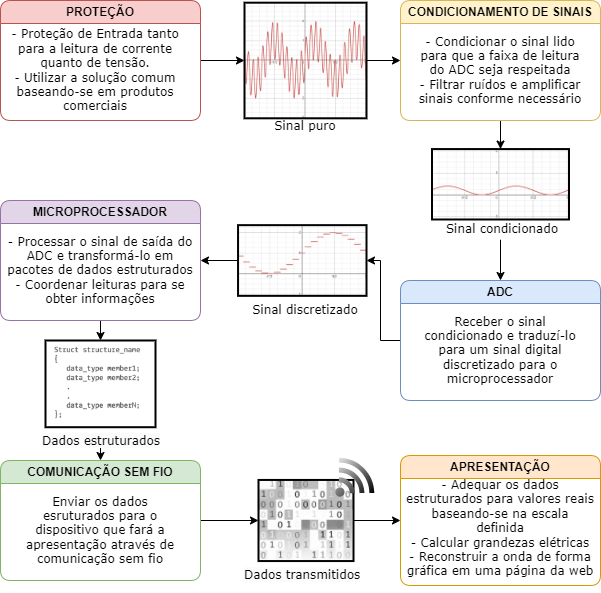
\includegraphics[width=1.0\textwidth]{figuras/dblocflux.png}
    \fonte{}
\end{figure}

Primeiramente, se tem a proteção de entrada. Esta é dividida em duas partes, sendo uma delas a proteção da entrada da tensão e a outra da corrente. Para se proteger a entrada de tensão, utilizam-se um resistor \gls{PTC} e \gls{MOV}s. O \gls{PTC} é projetado para caso a tensão de entrada do circuito seja muito maior que a desejada ou tenha um curto, este esquente e vire uma impedância muito grande, sendo assim uma barreira para qualquer tipo de corrente. Porém, a sua atuação para proteção é demasiada lenta, se pondo necessário a implementação dos \gls{MOV}s, que atuarão mais rapidamente e fecharão um curto entre a entrada e o ground do circuito enquanto o resistor está sendo ativado.

Para a proteção de corrente, primeiramente se é colocado fusíveis \gls{HRC}, que são fusíveis especiais para a extinção de qualquer possível arco voltaico decorrente da queima do filamento interno deste, prevenindo assim qualquer continuidade após a atuação deste. A ponte de diodos logo em seguida dos resistores shunt atua como um clamp de tensão para limitar esta caso ultrapasse de valores desejados e também como um caminho para a corrente, caso esta não seja o suficiente para queimar os fusíveis, mas sim para queimar o circuito. Estes componentes e sua montagem se encontram discretizados na \autoref{fig:circ-prot}

\begin{figure}[htb!]
    \caption{Entrada de Tensão e Corrente}
    \label{fig:circ-prot}
    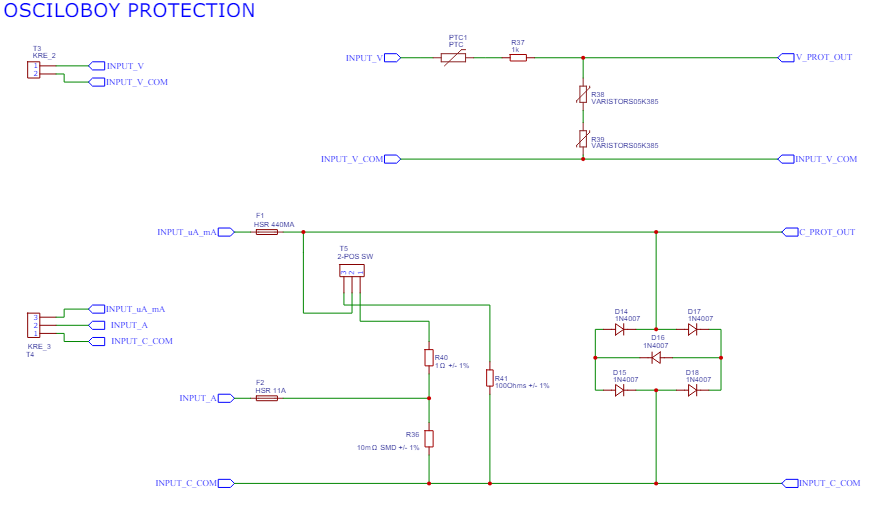
\includegraphics[width=0.8\textwidth]{figuras/circ-prot.png}
    \fonte{}
\end{figure}

Nesta figura também, pode-se observar as entradas do circuito, sendo a entrada de tensão diretamente ligada à próxima parte do circuito, sendo esta o condicionamento de sinais de tensão e a entrada de corrente composta por resistores, que servem como shunt para a leitura de corrente.

O resistor de 10 m$\Omega$ é para a leitura de corrente na proporção de Amperes, a série entre este e o resistor de 1 $\Omega$ compõe a leitura da entrada de mA e o resistor de 100 $\Omega$ para a leitura de $\mu$A. Para alternar entre as entradas de mA/$\mu$A e A, foi colocado um switch, discretizando-as.

Para se obter um sinal que o ADC consiga interpretar e também seja seguro para não queimá-lo, é de suma importância que este seja condicionado para tal, entrando na proxima parte do circuito, os condicionadores de tensão.

Existem duas possibilidades para a leitura de um sinal que \gls{ADC}s conseguem fazer: leitura "Diferencial" e leitura "\textit{Single-Ended}".

A primeira opção a ser considerada foi a \textit{Single-Ended}. Este tipo de leitura é feita pela comparação de tensão entre um ponto do circuito e o \textit{ground}. Para fazer tal leitura com diferentes \textit{ranges}, o que é de grande importância para se alcançar uma precisão boa, foi primeiro projetado um condicionamento de sinais por divisor resistivo, como representado na \autoref{fig:div-res}.

\begin{figure}[htb!]
    \caption{Condicionamento de sinais por divisor resistivo para leitura \textit{Single-Ended}}
    \label{fig:div-res}
    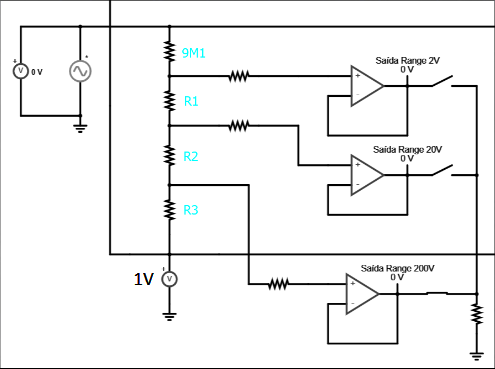
\includegraphics[width=0.6\textwidth]{figuras/div-res.png}
    \fonte{}
\end{figure}

Esta topografia promete 4 ranges de leitura tanto para corrente quanto para tensão, sendo estes 200 V, 20 V, 2 V e 200 mV (com precisão de 2\%) e 10 A, 200 mA, 20 mA e 2000 $\mu$A (com precisão de 5\%). É também necessário o uso de \gls{amp-op}s para a seleção do range, para isolar o \gls{ADC} da entrada e também para manter a tensão de entrada do \gls{ADC} dentro do range requerido.

Desta maneira, foram calculados os resistores de forma a manter a tensão de entrada dos \gls{amp-op}s sempre entre 30 e -30 V no maior fundo de escala possível (atenuação de 10x), respeitando os aspectos construtivos destes componentes. O cálculo para tais resistores se resume na resolução do seguinte sistema:

\begin{equation}
    \label{eq01}
    \begin{array}{lcl}
    \end{array}
\end{equation}

Obtendo os seguintes resultados:

\begin{equation}
    \label{eq02}
    \begin{array}{lcl}
    \end{array}
\end{equation}

Substituindo x, y e z, respectivamente, em R1, R2 e R3 na \autoref{fig:div-res}, chega-se às tensões condicionadas desejadas. Com isto, agora, é necessário serem respeitadas as necessidades do \gls{ADC}, que é o componente principal do circuito, pois este efetivamente fará as leituras.

Primeiramente, foi escolhido o \gls{ADC} ADS1115 da \textit{Texas Instruments}, pois este possui 16-bits de resolução, o que torna a leitura extremamente precisa, possui uma referência interna de tensão, tornando desnecessário a construção de uma referência no circuito, tornando-o menos complexo, além de ser compatível com o protocolo de comunicação \gls{$I^2$C} que será utilizado para interfacear este com o microcontrolador. Porém, devido a sua taxa de leitura extremamente baixa, de 860 \textit{samples per second}, ou \gls{SPS}, o que prejudicaria a leitura até de frequência 60 Hz, finalmente foi decidido se utilizar o \gls{ADC} ADS1015.

Este, também da \gls{TI}, apesar de ter uma resolução mais baixa de 12-bits, oferece uma taxa de \gls{SPS} de 3300, possibilitando assim uma reconstrução mais fiel da onda a ser lida,possuindo, como o ADS1115, uma referência interna de tensão e compatibilidade com o protocolo \gls{$I^2$C}. Este \gls{ADC} também possui uma proteção interna contra surtos por \gls{TVS}, tornando-o extremamente robusto. Os requerimentos para o funcionamento adequado deste \gls{ADC} são uma tensão de entrada máxima de 3,3 V e esta não pode ser negativa.

Seguindo tais parâmetros, nota-se que o condicionamento de sinal é inadequado, necessitando de mais componentes e circuitos auxiliares para exercer sua função adequadamente. Limitando-se a tensão de entrada a um range entre -1 e 1 V e adicionando um offset de tensão de 1 V para possibilitar a leitura de tensões negativas, se é imposto então que sinais entre 0 e 1 V serão interpretados como negativos e sinais entre 1 e 2 V a serem interpretados como positivos.

Para a leitura \textit{Single-Ended}, após o divisor resistivo e seu primeiro buffer, põe-se necessário, primeiramente, fazer uma inversão do sinal de \textit{output} do \gls{amp-op}, pois este inverte o sinal de entrada na saída, colocando em cascata um \gls{amp-op}. Para estes componentes conseguirem também suportar tensões negativas em sua entrada, é de grande importância que a sua alimentação seja simétrica. Isto acarreta na necessidade da utilização de mais um circuito auxiliar que possibilite a entrega desta tensão negativa, chamado \textit{Negative Charge Pump}.

Segundo, se é necessário também que a tensão de offset proposta seja de extrema precisão para introduzir o mínimo de erro possível ao sinal de leitura. Existem \gls{CI}s que exercem esta função com a precisão necessária, porém estes são extremamente caros.

Finalmente, para o menor range de tensão, seria necessária a aplicação de mais um \gls{amp-op} em cascata para a amplificação do sinal, pois este ficaria fora do range do bit menos significativo do \gls{ADC}, tornando o circuito de condicionamento de sinais algo como mostrado na \autoref{fig:cascata}.

\begin{figure}[htb!]
    \caption{Condicionamento de sinais por divisor resistivo para leitura \textit{Single-Ended}, menor range}
    \label{fig:cascata}
    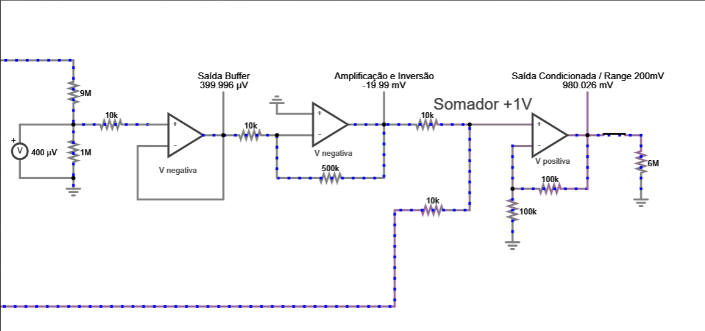
\includegraphics[width=0.6\textwidth]{figuras/cascata.png}
    \fonte{}
\end{figure}

Cada \gls{amp-op} possui um \textit{drift} de saída, o que introduz ainda mais erro à leitura do \gls{ADC}, além de como se é necessária uma amplificação de sinal final, quaisquer ruídos introduzidos serão também amplificados. Com todos estes problemas compostos, tomou-se a decisão de fazer a leitura por modo diferencial, que é a outra opção de leitura nativa ao \gls{ADC} escolhido.

Este tipo de leitura, ao invés de comparar a tensão entre um ponto do circuito e o \textit{ground}, compara a tensão entre dois pontos do circuito e mede efetivamente a diferença entre elas, como mostrado na \autoref{fig:difread}. Isso significa que nenhuma das entradas está ligada a uma referência, eliminando assim problemas referentes ao isolamento da leitura com o terra e também eliminando ruídos de entrada, pois como estes são introduzidos dos dois lados, eles se cancelam.

\begin{figure}[htb!]
    \caption{Condicionamento de sinais por divisor resistivo para leitura diferencial}
    \label{fig:difread}
    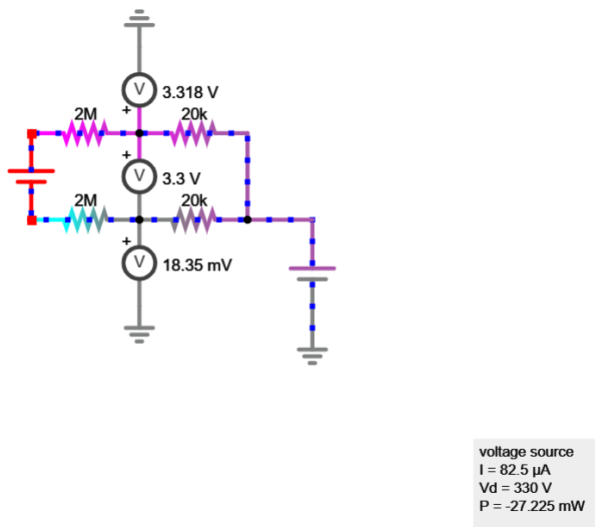
\includegraphics[width=0.6\textwidth]{figuras/difread.png}
    \fonte{}
\end{figure}

Para o dimensionamento dos resistores desta topologia, é feita uma malha resultando na seguinte equação:

\begin{equation}
    \label{eq03}
    \begin{array}{lcl}
    \end{array}
\end{equation}

Resolvendo esta, chega-se ao resultado de 2 M$\Omega$ e 20 k$\Omega$ para os resistores.

Para o offset de tensão, como os erros introduzidos são anulados pela própria topografia, utiliza-se uma referência tensão menos precisa, diminuindo o custo do circuito regulador como um todo. A referência de tensão utilizada para este projeto é fornecida pelo \gls{CI} TL431A, tendo este ainda assim uma precisão de 1\%, mas sendo muito mais barato que a opção anterior. Além disso, este possibilita mais facilmente a utilização do range inteiro de leitura do \gls{ADC}, tornando assim o offset $3,3/2$, que pode ser regulado pela ação do trimpot junto ao circuito auxiliar. Como não são utilizados \gls{amp-op}s, também não é necessária a utilização do circuito auxiliar \textit{Negative Charge Pump}.

Então, com todos estes benefícios em mente, foi escolhida esta topologia e tipo de leitura para o circuito final, como explícito na \autoref{fig:circ-cond-t}. Para a leitura de corrente, a mesma lógica se aplica, pois o resistor shunt é visto como uma fonte de tensão pelo circuito de leitura. Como esta tensão é extremamente baixa, não há a necessidade de um resistor de entrada para a atenuação da mesma, como explícito na \autoref{fig:circ-cond-c}.

\begin{figure}[htb!]
    \caption{Circuito de condicionamento de sinais para tensão}
    \label{fig:circ-cond-t}
    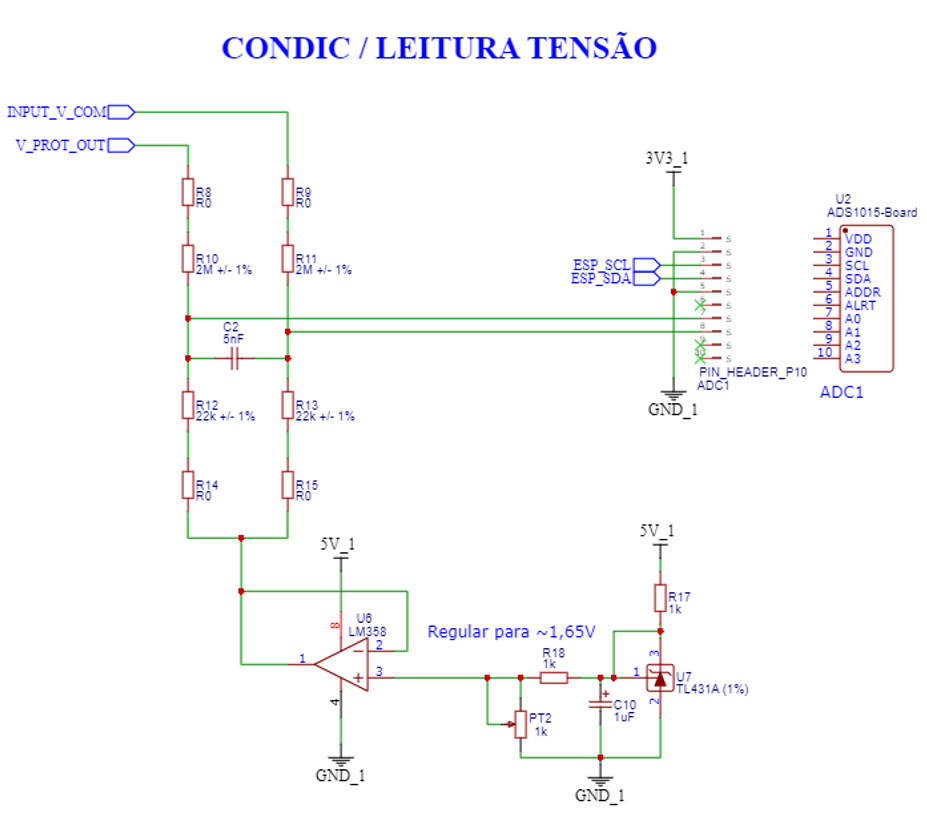
\includegraphics[width=0.6\textwidth]{figuras/circ-cond-t.png}
    \fonte{}
\end{figure}

\begin{figure}[htb!]
    \caption{Circuito de condicionamento de sinais para corrente}
    \label{fig:circ-cond-c}
    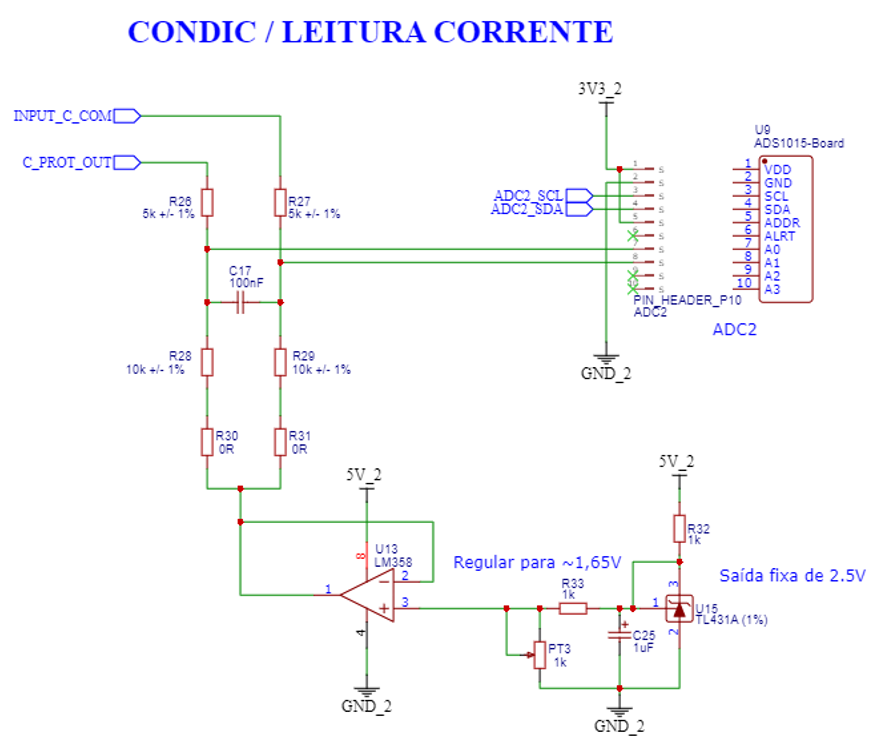
\includegraphics[width=0.6\textwidth]{figuras/circ-cond-c.png}
    \fonte{}
\end{figure}

Após a leitura dos sinais e a conversão feita pelo ADC, o sinal digital de saída é processado por um microcontrolador para então ser entregue a uma webpage e assim tratado para visualização pelo usuário. Algumas necessidades básicas devem ser atendidas pelo chip escolhido, como suporte para comunicação \textit{wireless}, seja \textit{WiFi} ou \textit{Bluetooth}, \textit{clock speed} alta o suficiente para não interferir na aquisição de dados e também ter uma boa documentação para ser possível o desenvolvimento do código.

Com isso em mente, o microcontrolador utilizado para este projeto é o ESP32, fabricado pela Espressif. A escolha deste foi feita por vários motivos:

\begin{itemize}
    \item Performance: O ESP32 opera em \textit{clock speeds} de até 240 MHz, oferecendo um robusto poder de processamento para o código e também para não interferir ou atrasar a aquisição dos sinais;
    \item Suporte: Este microcontrolador tem suporte tanto para \textit{WiFi} quanto para \textit{Bluetooth}, trabalha com o protocolo \gls{$I^2$C}, que será utilizado para fazer a comunicação tanto com o \gls{ADC} quanto com o webserver e utiliza-se do Arduino como sua principal plataforma de desenvolvimento;
    \item Ambiente: Este chip é extensamente utilizado em vários setores da tecnologia e tem uma vasta comunidade de usuários, o que garante um extenso leque de \textit{resources} como bibliotecas, tutoriais, videos, forums, entre outros, para ajudar na confecção do software e firmware. Também apresenta suporte oferecido pela própria Espressif sobre as suas funcionalidades muito bem documentados;
    \item Modularidade: Esta parte crucial do trabalho também é suportada por este microcontrolador, e
    \item Preço: Para todas as funcionalidades providas pelo ESP32, este apresenta um grande custo benefício, além de estar facilmente disponível no mercado.
\end{itemize}

Para ter uma comunicação confiável entre os dois \gls{ADC}s conectados a fontes diferentes e o ESP32, é necessário o isolamento entre estes, evitando-se curtos. Para isso, foi utilizado um circuito de comunicação isolada por optoacopladores, como demonstrado na \autoref{fig:circ-comunic}.

\begin{figure}[htb!]
    \caption{Circuito de comunicação isolado}
    \label{fig:circ-comunic}
    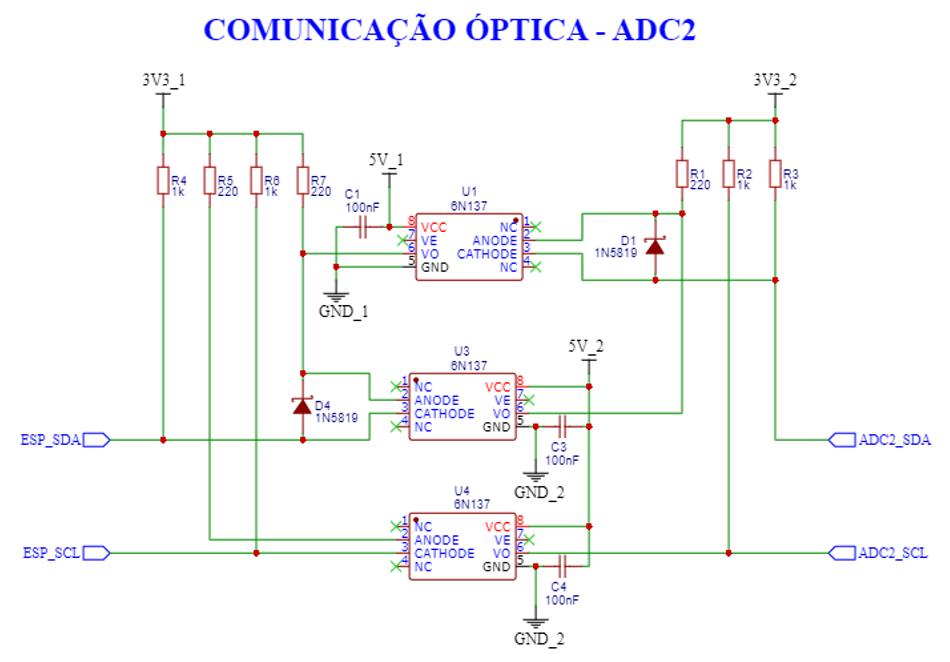
\includegraphics[width=0.6\textwidth]{figuras/circ-comunic.png}
    \fonte{}
\end{figure}

***explicação sobre o circuito de comunicação isolado e os optos***

Para a alimentação do circuito como um todo, existiam duas opções: baterias ou fontes. Como este protótipo será de bancada, foi escolhida a alimentação por fontes, pois estas não precisam ser trocadas frequentemente e é possível ligá-las à rede.

Para este projeto são utilizadas duas fontes isoladas, uma para alimentar o circuito de leitura de tensão e outra para alimentar o circuito de leitura de corrente, reduzindo assim possíveis ruídos e interferências entre circuitos e também aumentando a confiabilidade do protótipo, pois como o objetivo é realizar leituras simultâneas de corrente e tensão, um isolamento entre eles é necessário para prevenir curtos.

Porém, o output das fontes escolhidas é de 12 V, não atendendo as necessidades de alimentação dos \gls{CI}s envolvidos e também do microcontrolador. Para isso, circuitos de regulação de tensão foram implementados, gerando duas saídas, como explícito na \autoref{fig:circ-conv-T}. Estes circuitos são iguais tanto para a leitura de tensão e de corrente, visto que estes tem as mesmas necessidades.

\begin{figure}[htb!]
    \caption{Circuito de regulação de tensão}
    \label{fig:circ-conv-T}
    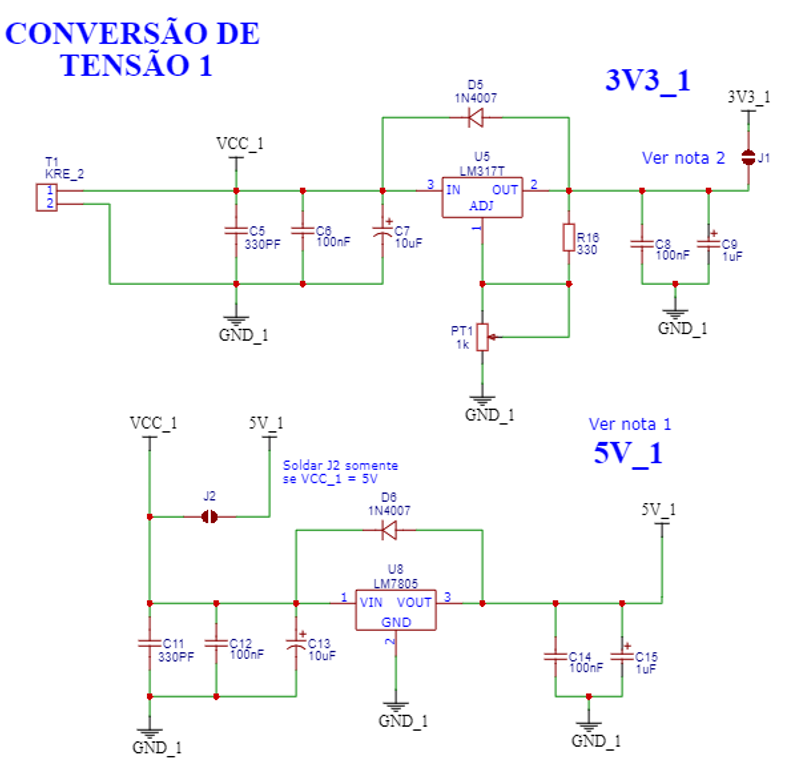
\includegraphics[width=0.6\textwidth]{figuras/circ-conv-T.png}
    \fonte{}
\end{figure}

Como visto na \autoref{fig:circ-cond-t}, o \gls{ADC} é alimentado com 3,3 V, mas o LM358 (que gera o offset de tensão) é alimentado com 5 V. O ESP32, como o \gls{ADC}, é alimentado com 3,3 V e esta está conectada, por especificação do projeto, sempre ao circuito de conversão de tensão referente à leitura de tensão.

\subsection{Software e Firmware}\label{softfirm}



\section{Materiais}\label{sec:materiais}

\begin{table}[!ht]
    \centering
    \caption{\textit{Book of Materials}}
    \label{tab:Bookofmaterials}
    \begin{tabular}{|l|l|l|}
        \hline
        \textbf{Material}                      & \textbf{Quantidade} & \textbf{Preço Unidade} \\ \hline
        \textbf{ESP32}                         & 01                  & N/A                    \\ \hline
        \textbf{ADC ADS1015}                   & 02                  & N/A                    \\ \hline
        \textbf{Buzzer THT}                    & 01                  & N/A                    \\ \hline
        \textbf{Capacitor 100 nF}              & 16                  & N/A                    \\ \hline
        \textbf{Capacitor 330 pF}              & 04                  & N/A                    \\ \hline
        \textbf{Capacitor 10 µF}               & 04                  & N/A                    \\ \hline
        \textbf{Capacitor 1 µF}                & 06                  & N/A                    \\ \hline
        \textbf{Diodo Schottky 1N5819}         & 04                  & N/A                    \\ \hline
        \textbf{Diodo 1N4007}                  & 10                  & N/A                    \\ \hline
        \textbf{Trimpot 1 K$\Omega$}           & 04                  & N/A                    \\ \hline
        \textbf{Transistor BC547}              & 01                  & N/A                    \\ \hline
        \textbf{Resistor 220 $\Omega$}         & 06                  & N/A                    \\ \hline
        \textbf{Resistor 1 k$\Omega$}          & 13                  & N/A                    \\ \hline
        \textbf{Resistor 330 $\Omega$}         & 02                  & N/A                    \\ \hline
        \textbf{Resistor 0 $\Omega$}           & 04                  & N/A                    \\ \hline
        \textbf{Resistor 3k3 $\Omega$}         & 01                  & N/A                    \\ \hline
        \textbf{Resistor 1\% 2 M$\Omega$}      & 04                  & N/A                    \\ \hline
        \textbf{Resistor 1\% 10 k$\Omega$}     & 04                  & N/A                    \\ \hline
        \textbf{Resistor 1\% 100 $\Omega$}     & 04                  & N/A                    \\ \hline
        \textbf{Resistor 1\% 1 $\Omega$}       & 04                  & N/A                    \\ \hline
        \textbf{Resistor SMD 1\% 10 m$\Omega$} & 01                  & N/A                    \\ \hline
        \textbf{Varistor S05K385}              & 02                  & N/A                    \\ \hline
        \textbf{Fusível HRC 440 mA}            & 01                  & N/A                    \\ \hline
        \textbf{Fusível HRC 11 A}              & 01                  & N/A                    \\ \hline
        \textbf{Borne KRE2}                    & 03                  & N/A                    \\ \hline
        \textbf{Borne KRE3}                    & 02                  & N/A                    \\ \hline
        \textbf{Alavanca 2 posições}           & 01                  & N/A                    \\ \hline
        \textbf{LM317T}                        & 02                  & N/A                    \\ \hline
        \textbf{LM358}                         & 02                  & N/A                    \\ \hline
        \textbf{LM7805}                        & 02                  & N/A                    \\ \hline
        \textbf{6N137}                         & 05                  & N/A                    \\ \hline
        \textbf{Barra de Pinos Fêmea 40x1}     & 02                  & N/A                    \\ \hline
        \textbf{PCB}                           & 01                  & N/A                    \\ \hline
        \textbf{Fonte Isolada}                 & 02                  & N/A                    \\ \hline
    \end{tabular}
\end{table}